
\FloatBarrier

\section{Synthetic Datasets}

\begin{figure}
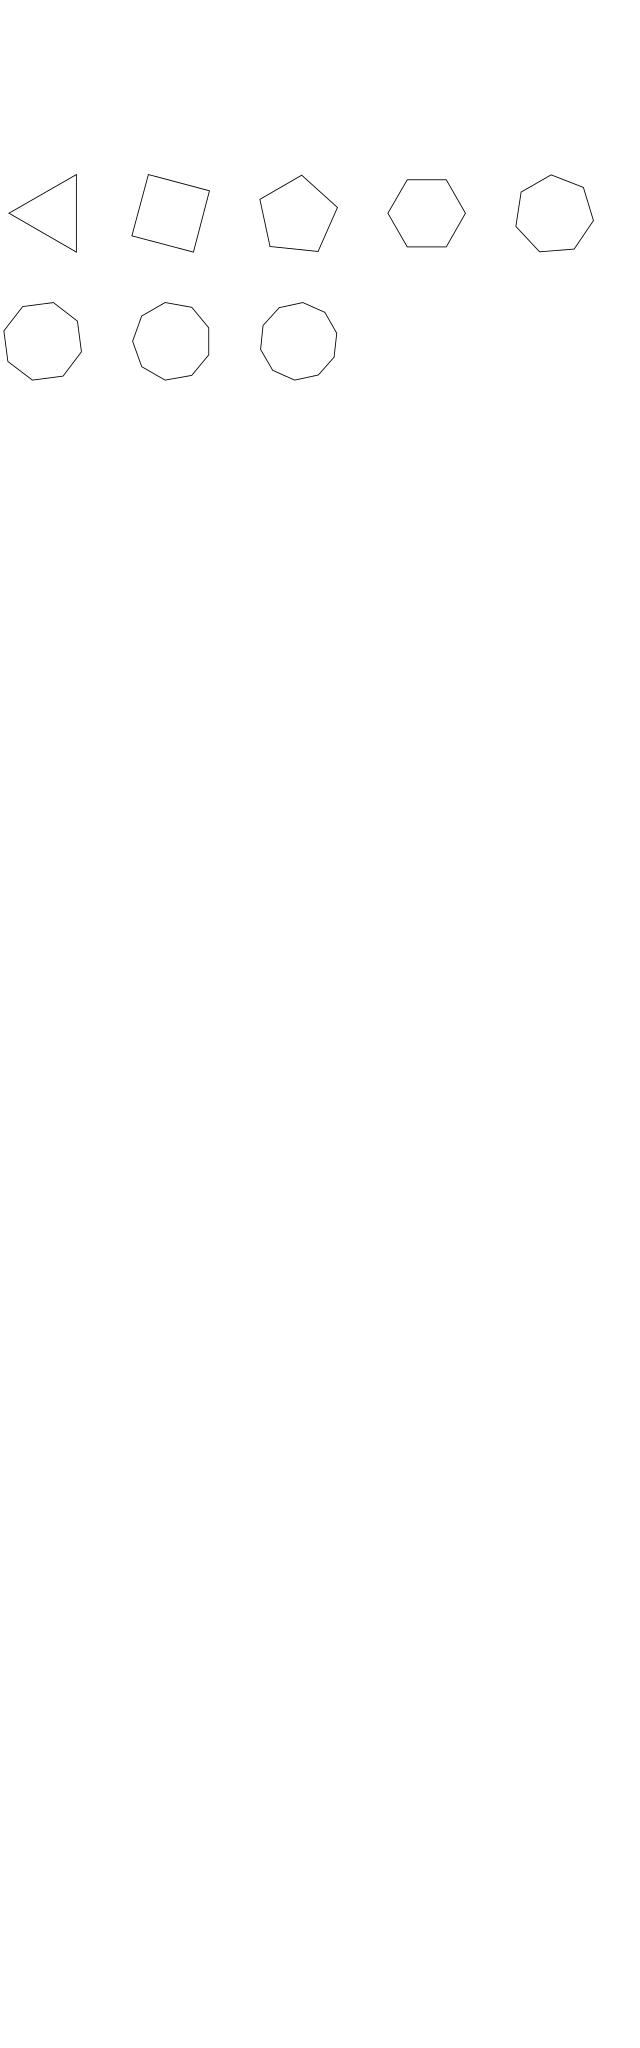
\includegraphics[width=\linewidth]{experiments/0.datasets/synth/output.d/polygons.png}
\caption{Polygons}
\end{figure}

\begin{figure}
\includegraphics[width=\linewidth]{experiments/0.datasets/synth/output.d/stars.png}
\caption{Stars}
\end{figure}

\begin{figure}
\includegraphics[width=\linewidth]{experiments/0.datasets/synth/output.d/articulator.png}
\caption{Articulator: A shape with an articulating arm}
\end{figure}

\begin{figure}
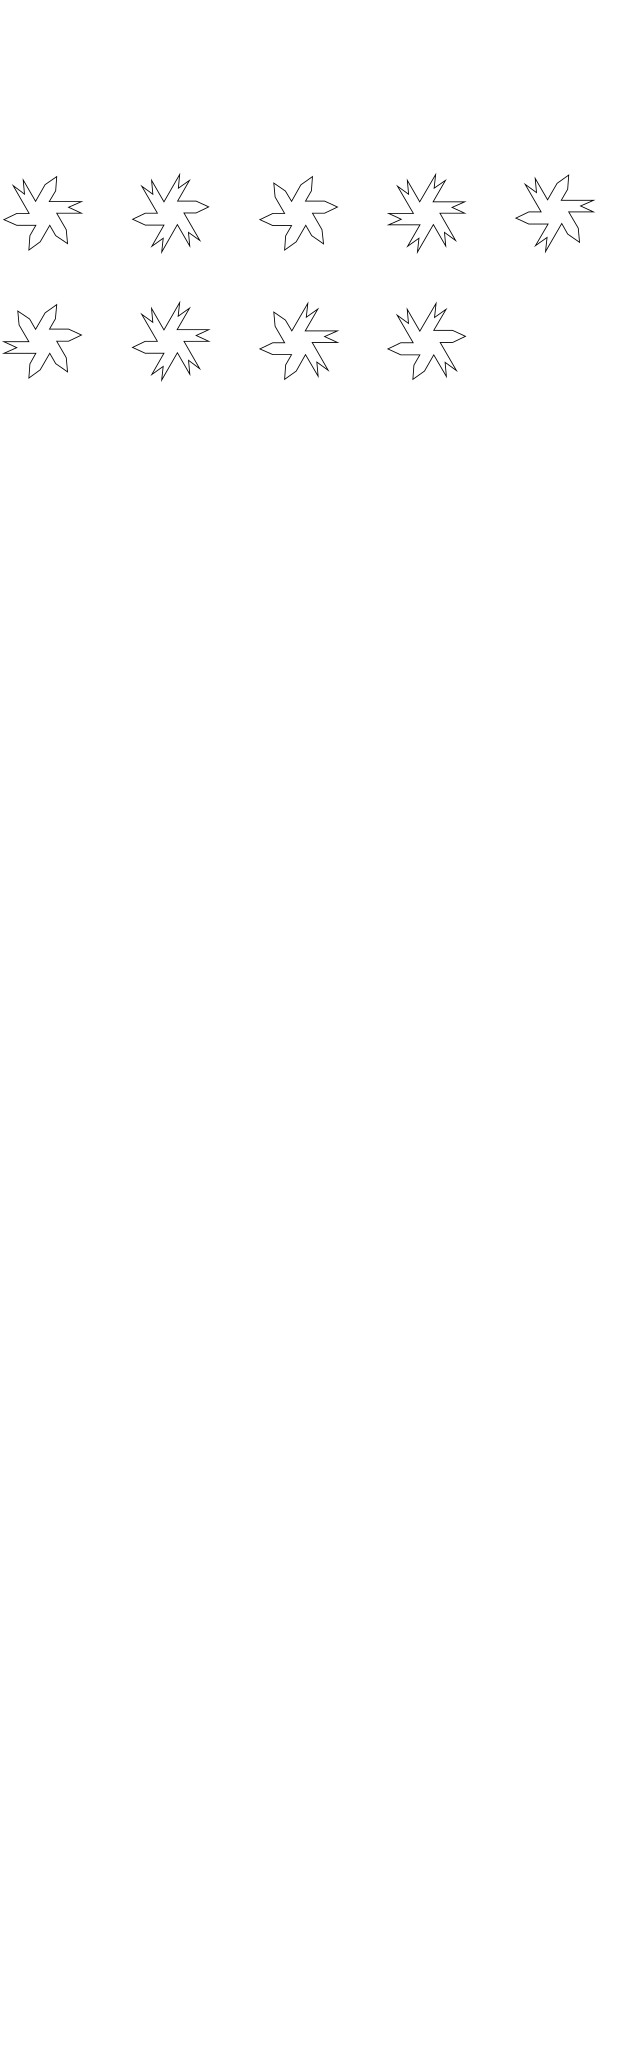
\includegraphics[width=\linewidth]{experiments/0.datasets/synth/output.d/narms.png}
\caption{These are 6-armed shapes, where each arm can have one of two shapes.}
\end{figure}